\documentclass[aspectratio=169,
hyperref={colorlinks,urlcolor=blue}
]{beamer}


%\usetheme{Pittsburgh}
\usetheme{default}
\usepackage{colortbl}%colored tables
%For using helvetica font:
\usepackage[scaled]{helvet}
\usepackage[T1]{fontenc}
\renewcommand\familydefault{\sfdefault}
\urlstyle{same} %sets the fonts for urls
\usepackage{pdfpages}
\usepackage{siunitx}
\usepackage{caption}
\usepackage{pifont}%for dings
\usepackage{pgfplots}%for 3d plotting
\pgfplotsset{compat = newest}
\usepackage{mathtools}%box in align env \Aboxed
\usepackage[american,smartlabels]{circuitikz}%for drawing circuits
\usepackage{multimedia}
\usepackage{animate}
\usepackage{xcolor}


\usetikzlibrary{arrows}
\usetikzlibrary {3d} 
\usetikzlibrary{decorations.markings, math}
\usetikzlibrary{intersections, pgfplots.fillbetween}
\usetikzlibrary {shapes.geometric} 


%\definecolor{myblue}{RGB}{5, 34, 150}
\definecolor{myblue2}{RGB}{5, 34, 150}
\definecolor{myblue}{RGB}{0,36,82}
\definecolor{myred}{RGB}{207, 2, 13}
\definecolor{mygreen}{RGB}{0, 158, 11}
\definecolor{myyellow}{RGB}{220,220,0}
\definecolor{qblue}{RGB}{0,36,82}
\definecolor{qgold}{RGB}{250,189,15}
\definecolor{qred}{RGB}{185,14,49}
\definecolor{cblue}{rgb}{0.13, 0.67, 0.8}
\definecolor{corange}{rgb}{0.8, 0.34, 0.0}
\definecolor{cpurple}{rgb}{0.54, 0.29, 0.42}

%%%%%%%%%%%% General settings
\setbeamercolor{frametitle}{fg=black}
\setbeamercolor{title}{fg=black}
\setbeamercolor{author}{fg=myblue2}

\beamertemplatenavigationsymbolsempty %no navigation controls at bottom of slides
%\setbeamertemplate{footline}[frame number]
\usefonttheme{professionalfonts} 
\setbeamerfont{title}{series=\bfseries,parent=structure}
\setbeamerfont{frametitle}{series=\bfseries,parent=structure}

%%%%%%%%%%%%Lists
\setbeamertemplate{itemize item}[circle] %{\color{myblue}$\circ$}
\setbeamertemplate{itemize subitem}{\color{myblue2}$\circ$}
\setbeamertemplate{itemize subsubitem}{\color{myblue2}$\cdot$}
\setbeamercolor{itemize item}{bg=myblue2,fg=myblue2}
\setbeamercolor{enumerate item}{bg=myblue2,fg=myblue2}
%%%%%%%%%%%%%%%%%%%%%%%%%%%%

%%%%%%%%%%%%Blocks
\setbeamertemplate{blocks}[rounded]
%Default block
\setbeamercolor{block title}{bg=myblue2, fg=white}
\setbeamercolor{block body}{bg=myblue2!10}
\setbeamerfont{block body}{size=\scriptsize}
\setbeamerfont{block title}{size=\scriptsize}
%Alert block
\setbeamercolor{block title alerted}{bg= myblue2, fg=white}
\setbeamercolor{block body alerted}{bg=myblue2!10}
\setbeamerfont{block body alerted}{size=\scriptsize}
\setbeamerfont{block title alerted}{size=\scriptsize}
%example block
\setbeamercolor{block title example}{bg=mygreen, fg=white}
\setbeamercolor{block body example}{bg=mygreen!10}
\setbeamerfont{block body example}{size=\scriptsize}
\setbeamerfont{block title example}{size=\scriptsize}
%%%%%%%%%%%%%%%%55


%%%%%%%%%%%%Figures and captions
\captionsetup{font=scriptsize,labelfont=scriptsize}
%\setbeamertemplate{caption}{\raggedright\insertcaption\par}
\newenvironment{capfig}[3]{\begin{figure}\includegraphics[width=#1\textwidth]{#2}\caption*{\textit{#3}}\end{figure}}{}

%\makeatother
%\setbeamertemplate{footline}
%{
%  \leavevmode%
%  \hbox{%
%  \begin{beamercolorbox}[wd=.4\paperwidth,ht=2.25ex,dp=1ex,center]{author in head/foot}%
%    \usebeamerfont{author in head/foot}\insertshortauthor
%  \end{beamercolorbox}%
%  \begin{beamercolorbox}[wd=.6\paperwidth,ht=2.25ex,dp=1ex,center]{title in head/foot}%
%    \usebeamerfont{title in head/foot}\insertshorttitle\hspace*{3em}
%    \insertframenumber{} / \inserttotalframenumber\hspace*{1ex}
%  \end{beamercolorbox}
%  }%
%  \vskip0pt%
%}
%\makeatletter

\makeatother
\setbeamertemplate{footline}
{
  \leavevmode%
  \hbox{%
\begin{beamercolorbox}[wd=.27\paperwidth,ht=2.25ex,dp=1ex,center]{author in head/foot}%
    \color{black}{\insertinstitute}
\end{beamercolorbox}
  \begin{beamercolorbox}[wd=.27\paperwidth,ht=2.25ex,dp=1ex,center]{author in head/foot}%
    \color{black}{\inserttitle}
  \end{beamercolorbox}%
  \begin{beamercolorbox}[wd=.27\paperwidth,ht=2.25ex,dp=1ex,center]{title in head/foot}%
    \color{black}{\insertshortauthor}
  \end{beamercolorbox}
  \begin{beamercolorbox}[wd=.27\paperwidth,ht=2.25ex,dp=1ex,center]{title in head/foot}%
    \hspace{.28\paperwidth}\color{black} \insertframenumber{} / \inserttotalframenumber\hspace*{1ex}
  \end{beamercolorbox}
  }%
  \vskip0pt%
}
\makeatletter

\setbeamertemplate{title page}
{
  \begin{tikzpicture}[remember picture,overlay]
    \def\barh{4}%15
  
    \draw[color=myblue2,line width=\barh] ([yshift=-0.5*\barh]current page.north west) -- ([yshift=-0.5*\barh,xshift=-0.67\paperwidth]current page.north east);
    \draw[color=myblue2,line width=\barh] ([yshift=-0.5*\barh,xshift=-0.67\paperwidth]current page.north east) -- ([yshift=-0.5*\barh,xshift=-0.34\paperwidth]current page.north east);
    \draw[color=myblue2,line width=\barh] ([yshift=-0.5*\barh,xshift=-0.34\paperwidth]current page.north east) -- ([yshift=-0.5*\barh]current page.north east); 
  
    \draw[color=myblue2,line width=\barh] ([yshift=0.5*\barh]current page.south west) -- ([yshift=0.5*\barh,xshift=-0.67\paperwidth]current page.south east);
    \draw[color=myblue2,line width=\barh] ([yshift=0.5*\barh,xshift=-0.67\paperwidth]current page.south east) -- ([yshift=0.5*\barh,xshift=-0.34\paperwidth]current page.south east);
    \draw[color=myblue2,line width=\barh] ([yshift=0.5*\barh,xshift=-0.34\paperwidth]current page.south east) -- ([yshift=0.5*\barh]current page.south east);
    %\node[left] at (current page.east) {
    %
\includegraphics[scale=0.1]{figures/coverpage}
    %};
  \end{tikzpicture}
  
  \usebeamerfont{title}\usebeamercolor[fg]{title}\inserttitle\par
  \usebeamerfont{subtitle}\usebeamercolor[fg]{subtitle}\insertsubtitle\par
  \vspace{2cm}
  \usebeamerfont{author}\usebeamercolor[fg]{author}\insertauthor\par
  \usebeamerfont{institute}\usebeamercolor[fg]{author}\insertinstitute\par
  \usebeamercolor[fg]{author}\par
  \usebeamercolor[fg]{titlegraphic}\inserttitlegraphic

} 

\setbeamertemplate{frametitle}{%
    \nointerlineskip%
        \par\hspace*{-\dimexpr0.5\paperwidth-0.5\textwidth}\textcolor{myblue2}{\rule{0.33\paperwidth}{6pt}}\textcolor{myblue2}{\rule{0.33\paperwidth}{6pt}}\textcolor{myblue2}{\rule{0.34\paperwidth}{6pt}} 
    \begin{beamercolorbox}[wd=\paperwidth,ht=0.75cm,dp=0.6ex]{frametitle}
        \hspace*{0.5cm}\strut\usebeamerfont{frametitle}\insertframetitle\strut
        %\hrule
    \end{beamercolorbox}%
    %%Line below:
%\par\hspace*{-\dimexpr0.5\paperwidth-0.5\textwidth}\textcolor{myblue}{\rule{\paperwidth}{0.4pt}}
     % <-- calculation of left margin width + rule
     %\textcolor{red}{\noindent\rule{\paperwidth}{2pt}}
}


%%%%%%%%%%%%Frame templates

%Slide with title
\newenvironment{titleframe}[1]
{\begin{frame}\frametitle{#1}\end{frame}}
{}

%Slide with title and itemize list:
\newenvironment{bulletframe}[1]
{\begin{frame}{#1} \itemize}
{\enditemize \end{frame}}

%Slide with two columns 50/50
\newenvironment{twocolframe}[3]
{\begin{frame}{#1}
 \begin{columns}[T]
 \column{0.5\textwidth}#2
 \column{0.5\textwidth}#3
 \end{columns}\end{frame}}{}

%Slide with two columns 60/40 <<<<<<<<<<<<<<<<<<<<<<  This one!
\newenvironment{twocolframesf}[3]
{\begin{frame}{#1}
 \begin{columns}[T]
 \column{0.6\textwidth}#2
 \column{0.4\textwidth}#3
 \end{columns}\end{frame}}{}
 
%Slide with two columns 70/30
\newenvironment{twocolframest}[3]
{\begin{frame}{#1}
 \begin{columns}[T] 
 \column{0.7\textwidth}#2
 \column{0.3\textwidth}#3
 \end{columns}\end{frame}}{} 
 
%Slide with two columns 40/60
\newenvironment{twocolframefs}[3]
{\begin{frame}{#1}
 \begin{columns}[T] 
 \column{0.4\textwidth}#2
 \column{0.6\textwidth}#3
 \end{columns}\end{frame}}{}
 
%Slide with two columns 70/30
\newenvironment{twocolframets}[3]
{\begin{frame}{#1}
 \begin{columns}[T] 
 \column{0.3\textwidth}#2
 \column{0.7\textwidth}#3
 \end{columns}\end{frame}}{} 

 
%Colloquium speaker (title, abstract, picture file, speaker name)
\newenvironment{colloquium}[5]
{
\begin{frame}{Colloquium: Friday 1:30pm in Stirling A}
\begin{columns}[T] 
 \column{0.8\textwidth}
 \textbf{#1}\\
 #2
 \column{0.2\textwidth}
 \capfig{#3}{#4}{#5}
 \end{columns}
\end{frame}
}
{} 

%%%%%%%%%%%%%Set Hyperref colors


\hypersetup{
  colorlinks=true,
  linkcolor=blue,    
  urlcolor=blue,     
  citecolor=blue      
}
%%%%%%%%%%%%%TOC bolding
\setbeamerfont{section in toc}{series=\bfseries}



%Frames:
% \twocolframesf 60/40 (fs, st, ts) 
% \titleframe
% bulletframe


%%%%%%%%%%%%%%%%%%%%%%%%%
%%%%%% START OF PRESENTATION %%%%%%
%%%%%%%%%%%%%%%%%%%%%%%%%

\title{Gravity}
\subject{Kepler, Newton, Gauss and Einstein}
\subtitle{Building Models to Describe our World}


\begin{document}

%%%%%%%%%%%%%%%%%%%%%%%%%
%%%%%% Title slide %%%%%%
%%%%%%%%%%%%%%%%%%%%%%%%%
\chaptertitle{Gravity}
\begin{frame}
\titlepage
\thispagestyle{empty}

\begin{textblock*}{5cm}(11cm,4cm)
    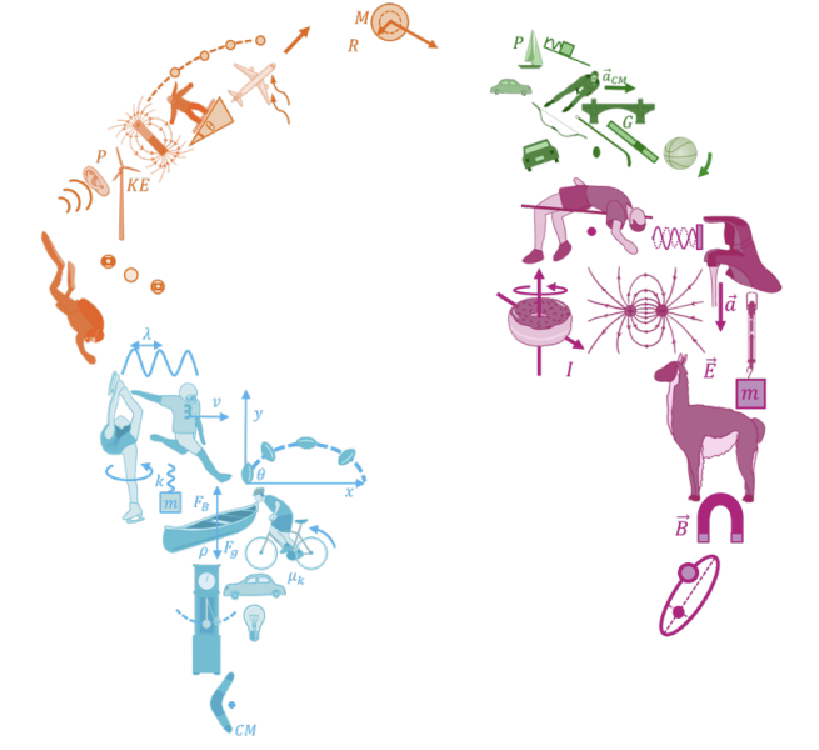
\includegraphics[width=4cm]{figures/BMDW/logo}
\end{textblock*}

\end{frame}

%%%%%%%%%%%%%%





\twocolframe{Outline}
{\tableofcontents[sections=1, subsectionstyle=show/show]\thispagestyle{empty}}
{\tableofcontents[sections=2-3, subsectionstyle=show/show]}





%%%%%%%%%%%%%%%%%%%%%

\section{Keplerian and Newtonian Gravity}
\label{sec:keplernnewtongravity}
\title{Keplerian and Newtonian Gravity}


%%%%%%%%%%%%%%%%%%%%%%%%%
\begin{frame}
\titlepage
\thispagestyle{empty}
\end{frame}

%%%%%%%%%%%%%%%%%%%%%%





\subsection{Kepler's laws}
\label{subsec:keplerslaws}
\begin{frame}{Kepler's Laws}
\begin{enumerate}
\item The path of a planet around the Sun is described by an ellipse with the Sun at one of its foci.
\item All planets move in such a way that the area swept by a line connecting the planet and the Sun in a given period of time is constant.
\item The ratio between the orbital periods, $T$, of two planets squared is equal to the ratio of the semi-major axes, $s$, of their orbits cubed:
\begin{align*}
\left( \frac{T_1}{T_2}\right)^2=\left( \frac{s_1}{s_2}\right)^3
\end{align*}
\end{enumerate}

\end{frame}


%%%%%%%%%%%%%%%%%%%%%%%%%%%%%%%%

%%%%%%%%%%%%%%%%%%%%%%%%%%%%%%%%
\subsubsection{First law}
\label{subsubsec:firstlaw}
\twocolframe{Kepler's First Law}
{
\begin{itemize}
\item Orbits of planets are ellipses (but some bodies that are not in bound orbits will have parabolic or hyperbolic orbits).
\item Ellipses are characterized by the location of two foci and one dimension (e.g. semi-major/minor axis, eccentricity).
\end{itemize}
\begin{align*}
\frac{x^2}{s^2}+\frac{y^2}{b^2}&=1\\
e&=\sqrt{s^2-b^2}\quad(s\geq b)
\end{align*}
}
{
\vspace{-1cm}
\begin{center}
\begin{tikzpicture}
\tikzmath{
\a=2.5;
\b=1.25;
\c=sqrt(\a*\a-\b*\b);
\xe=\a/2;
\ye=\b/2*sqrt(3);
\ae=0.5*\a;
\be=0.7*\b;
\ce=sqrt(\ae*\ae-\be*\be);
\xm=\xe+\ce+\ae/2;
\ym=\ye+\be/2*sqrt(3);
}

\scalebox{1}{
\draw (0,0) ellipse ({\a} and \b);

\draw[latex-latex, line width=1,color=myred] (0,0) -- +(0,\b) node[midway,right]{\scriptsize semi-minor axis, $b$};
\draw[latex-latex, line width=1,color=myred] (0,0) -- +(-\a,0) node[midway,above]{\scriptsize semi-major axis, $s$};
\draw[latex-latex, line width=1,color=myblue!60] (0,0) -- +(\c,0) node[midway,above]{\scriptsize eccentricity, $e$};
\fill (-\c,0) circle(2pt) node[below right]{\scriptsize Focus};
\fill (\c,0) circle(2pt) node[below left]{\scriptsize Focus};

\begin{scope}[shift={(0,-3.5)}]
\draw (0,0) ellipse ({\a} and \b);
\node at (-\c,0)  {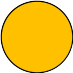
\includegraphics[scale=0.15]{figures/Gravity/sun}};
\node at (\xe,\ye)  {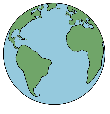
\includegraphics[scale=0.1]{figures/Gravity/earth}};
\draw (\xe+\ce,\ye) ellipse ({\ae} and \be);
\node at (\xm,\ym)  {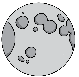
\includegraphics[scale=0.1]{figures/Gravity/moon}};
\fill (-\a,0) circle(2pt) node[left]{\scriptsize perihelion};
\fill (\a,0) circle(2pt) node[left]{\scriptsize aphelion};
\fill (\xe+\ce-\ae,\ye) circle(2pt) node[left]{\scriptsize perigee};
\fill (\xe+\ce+\ae,\ye) circle(2pt) node[left]{\scriptsize apogee};
\end{scope}

}

\end{tikzpicture}
\captionof*{figure}{\textit{Elliptical orbits and their parameters.}}
\end{center}

}

%%%%%%%%%%%%%%%%%%%%%%%%%%%%%%%%
\subsubsection{Second law}
\label{subsubsec:secondlaw}
\twocolframe{Kepler's Second Law}
{
\begin{itemize}
\item ``Equal areas swept out in equal times'':
\begin{itemize}
\item[$\rightarrow$] Planets move faster near the perihelion.
\item[$\rightarrow$] Bodies in a circular orbit move at constant speed.
\end{itemize}

\end{itemize}
}
{

\begin{center}
\begin{tikzpicture}
\tikzmath{
\a=2.5;
\b=1.5;
\c=sqrt(\a*\a-\b*\b);
\tA=20;
\tB=\tA+20;
\tC=110;
\tD=\tC+40;
\Ax=\a*cos(\tA);
\Ay=\b*sin(\tA);
\Bx=\a*cos(\tB);
\By=\b*sin(\tB);
\Cx=\a*cos(\tC);
\Cy=\b*sin(\tC);
\Dx=\a*cos(\tD);
\Dy=\b*sin(\tD);
\thA=atan(\Ay/\Ax);
\thB=atan(\By/\Bx);
\Ar=1.1*sqrt(\Ax*\Ax+\Ay*\Ay);
\Br=1.1*sqrt(\Bx*\Bx+\By*\By);
\Cr=1.1*sqrt(\Cx*\Cx+\Cy*\Cy);
\Dr=1.1*sqrt(\Dx*\Dx+\Dy*\Dy);
\biga=1.3*\a;
\bigb=1.3*\b;
}

\scalebox{1}{

\coordinate (A) at (\Ax,\Ay);
\coordinate (B) at (\Bx,\By);
\coordinate (C) at (\Cx,\Cy);
\coordinate (D) at (\Dx,\Dy);

\begin{scope}
\clip (0,0) ellipse ({\a} and \b);
\fill[color=myblue!40] (-\c,0) -- (\thA:\Ar) -- (\thB:\Br) --cycle;
\fill[color=myblue!40] (-\c,0) -- (\tC:\Cr) -- (\tD:\Dr) --cycle;
\end{scope}

\draw (0,0) ellipse ({\a} and \b);


\fill (A) circle(2pt) node[above, right]{$A$};
\fill (B) circle(2pt) node[above]{$B$};
\fill (C) circle(2pt) node[above]{$C$};
\fill (D) circle(2pt) node[left]{$D$};

\node at (-\c,0)  {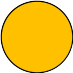
\includegraphics[scale=0.15]{figures/Gravity/sun}};

\draw [-latex, dashed] (\biga,0) arc(0:180:{\biga} and \bigb) node[midway,above]{\scriptsize motion of planet};



}

\end{tikzpicture}
\captionof*{figure}{\textit{Planets sweep out equal areas in equal amounts of time.}}
\end{center}

}


%%%%%%%%%%%%%%%%%%%%%%%%%%%%%%%%
\subsubsection{Third law}
\label{subsubsec:thirdlaw}
\twocolframe{Kepler's Third Law}
{
\begin{itemize}
\item The ratio between the orbital periods, $T$, of two planets squared is equal to the ratio of the semi-major axes, $s$, of their orbits cubed:
\begin{align*}
\left( \frac{T_1}{T_2}\right)^2=\left( \frac{s_1}{s_2}\right)^3
\end{align*}
\item It's a mouthful... But it just means that:
\begin{align*}
\frac{T^2}{s^3}=\text{constant}
\end{align*}
\end{itemize}

}
{

\begin{center}
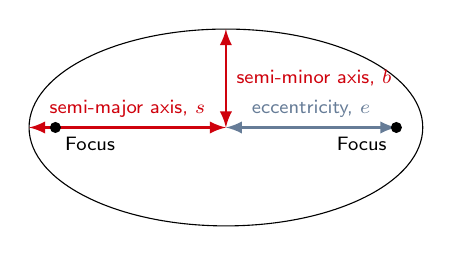
\begin{tikzpicture}
\tikzmath{
\a=2.5;
\b=1.25;
\c=sqrt(\a*\a-\b*\b);
\xe=\a/2;
\ye=\b/2*sqrt(3);
\ae=0.5*\a;
\be=0.7*\b;
\ce=sqrt(\ae*\ae-\be*\be);
\xm=\xe+\ce+\ae/2;
\ym=\ye+\be/2*sqrt(3);
}

\scalebox{1}{
\draw (0,0) ellipse ({\a} and \b);

\draw[latex-latex, line width=1,color=myred] (0,0) -- +(0,\b) node[midway,right]{\scriptsize semi-minor axis, $b$};
\draw[latex-latex, line width=1,color=myred] (0,0) -- +(-\a,0) node[midway,above]{\scriptsize semi-major axis, $s$};
\draw[latex-latex, line width=1,color=myblue!60] (0,0) -- +(\c,0) node[midway,above]{\scriptsize eccentricity, $e$};
\fill (-\c,0) circle(2pt) node[below right]{\scriptsize Focus};
\fill (\c,0) circle(2pt) node[below left]{\scriptsize Focus};

}

\end{tikzpicture}
\captionof*{figure}{\textit{Kepler's Third Law relates to the semi-major axis.}}
\end{center}
\textit{That constant depends on the mass of the body that the planets orbit (e.g. the Sun). Thus, by measuring $T$ and $s$, you can determine the mass of the Sun!}
}


%%%%%%%%%%%%%%%%%%%%%%%%%%%%%%%%
\subsection{Newton's theory of gravity}
\label{subsec:newtonstheoryofgravity}
\begin{frame}{Newton's Universal Theory of Gravity (magnitude)}
\begin{itemize}
\item Two bodies with mass will exert an \textbf{attractive} force on each other that is proportional to the \textbf{product of their masses} and inversely proportional to the \textbf{distance between them squared}:
\begin{align*}
F \propto \frac{M_1M_2}{r^2}
\end{align*}
\item The constant of proportionality is called the gravitational constant, $G$:
\begin{align*}
F =G \frac{M_1M_2}{r^2}
\end{align*}
\end{itemize}
\end{frame}


%%%%%%%%%%%%%%%%%%%%%%%%%%%%%%%%
\subsubsection{The Cavendish experiment}
\label{subsubsec:thecavendishexperiment}
\twocolframesf{The Cavendish experiment}
{
\begin{itemize}
\item Want to measure G.
\item The forces involved are minuscule (less than \num{1e-6} Newtons).
\item Clever use of a ``torsion pendulum'': two masses suspended by a thin fibre.
\item Bring two big masses close to the suspended masses and measure by how much they twist.
\item Very sensitive experiment... 
\end{itemize}
}
{
\capfig{1}{figures/Gravity/cavendish}{Figure from Cavendish's paper showing the torsion pendulum and building it was housed in. The large masses could be rotated from the outside through a system of pulleys. Philosophical Transactions of the Royal Society of London, (part II) \textbf{88} p.469-526 (21 June 1798).}
}


%%%%%%%%%%%%%%%%%%%%%%%%%%%%%%%%


%%%%%%%%%%%%%%%%%%%%%%%%%%%%%%%%
\subsubsection{Magnitude and direction}
\label{subsec:magnitudeanddirection}
\twocolframesf{Newton's Universal Theory of Gravity (magnitude and direction)}
{
The force, $\vec F_{12}$, \textbf{on} mass $M_1$ \textbf{from} $M_2$ can be written as:
\begin{align*}
\vec F_{12} = - G \frac{M_1M_2}{r_{12}^2}\hat r_{12}=-G \frac{M_1M_2}{r_{12}^{\textcolor{myred}{3}}} \textcolor{myred}{\vec r_{12}}
\end{align*}
where:
\begin{align*}
\vec r_{12}=\vec r_1 - \vec r_2\;\;\text{and}\;\; \hat r_{12}=\frac{\vec r_{12}}{r_{12}}
\end{align*}
In general, we use the \textbf{minus sign to indicate that the force is attractive} (we could've used a plus sign and the vector $\vec r_2 -\vec r_1$, but we don't!).
}
{
\begin{center}
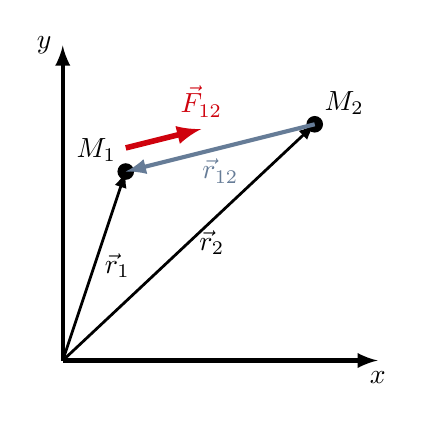
\begin{tikzpicture}
\tikzmath{
\L=4;
}
\scalebox{1}{

\coordinate (M1) at (0.2*\L, 0.6*\L);
\coordinate (M2) at (0.8*\L, 0.75*\L);

\draw[-latex,line width=1.5] (0,0) -- (\L,0) node[below]{$x$};
\draw[-latex,line width=1.5] (0,0) -- (0,\L) node[left]{$y$};

\fill (M1) circle (3pt) node[above left]{$M_1$};
\fill (M2) circle (3pt) node[above right]{$M_2$};

\draw[-latex,line width=1] (0,0) -- (M1) node[midway,right] {$\vec r_1$};
\draw[-latex,line width=1] (0,0) -- (M2) node[midway,right] {$\vec r_2$};

\draw[-latex,line width=2, color=myred] ($(M1)+(0,0.3)$) -- ($(M1)!0.4!(M2)+(0,0.3)$) node[above] {$\vec F_{12}$};
\draw[-latex,line width=1.5, color=myblue!60] (M2) -- (M1) node[midway,below] {$\vec r_{12}$};

}

\end{tikzpicture}
\captionof*{figure}{\textit{Vectors in Newton's Universal Theory of Gravity. The force on $M_1$ is in the opposite direction of $\vec r_{12}$.}}
\end{center}
}


%%%%%%%%%%%%%%%%%%%%%%%%%%%%%%%%

%%%%%%%%%%%%%%%%%%%%%%%%%%%%%%%%
\subsubsection{M > > > m}
\label{subsubsec:mmuchgreaterthanm}
\twocolframesf{When one mass is much larger}
{
\begin{itemize}
\item If $M$ is much bigger than $m$, $M$ can be considered as effectively stationary (e.g. the Sun when considering the motion of planets, the Earth when considering the motion of satellites).
\item Makes sense to make $M$ the origin of our coordinate system, so the force on $m$ (at position, $\vec r$ is):
\begin{align*}
\vec F = - G \frac{Mm}{r^2}\hat r= - G \frac{Mm}{r^3}\vec r
\end{align*}
\end{itemize}
}
{
\begin{center}
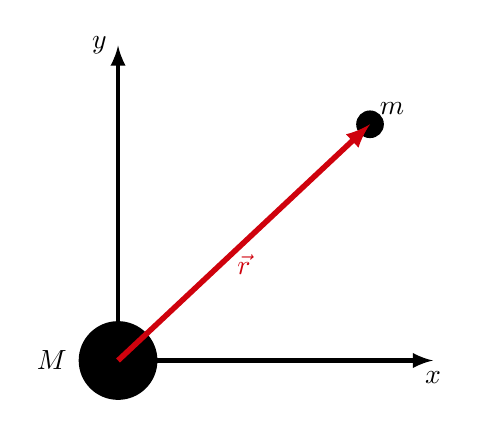
\begin{tikzpicture}
\tikzmath{
\L=4;
}
\scalebox{1}{

\coordinate (M) at (0,0);
\coordinate (m) at (0.8*\L, 0.75*\L);

\draw[-latex,line width=1.5] (0,0) -- (\L,0) node[below]{$x$};
\draw[-latex,line width=1.5] (0,0) -- (0,\L) node[left]{$y$};

\fill (M) circle (0.5) node[left=15pt]{$M$};
\fill (m) circle (5pt) node[above right]{$m$};

\draw[color=myred,-latex,line width=2] (M) -- (m) node[midway,below] {$\vec r$};

}

\end{tikzpicture}
\captionof*{figure}{\textit{Newton's Universal Theory of Gravity with one mass at the origin.}}
\end{center}
}


%%%%%%%%%%%%%%%%%%%%%%%%%%%%%%%%
\subsection{The constant from Kepler's third law}
\label{subsec:thecnstfromkeplersthirdlaw}
\twocolframe{The constant from Kepler's Third Law}
{
\vspace{-0.25cm}
\begin{itemize}
\item The constant is given by:
\begin{align*}
\frac{T^2}{s^3}=\text{constant}
\end{align*}
\item<2-> Can evaluate this using a circular orbit:
\begin{align*}%
G\frac{Mm}{r^2}=m\frac{v^2}{r}\;\;&\rightarrow\;\; v=\sqrt{\frac{GM}{r}}\\%
v=\frac{2\pi r}{T}\;\;&\rightarrow\;\;T=\frac{2\pi r}{v}=\frac{2\pi r}{\sqrt{\frac{GM}{r}}} %
\end{align*}%
\item<3-> The constant is then given by:
\begin{align*}
\frac{T^2}{r^3}=\frac{4\pi^2 r^2}{r^3\frac{GM}{r}}=\frac{4\pi^2}{GM}
\end{align*}
\end{itemize}

}
{
\vspace{-0.5cm}
\begin{center}
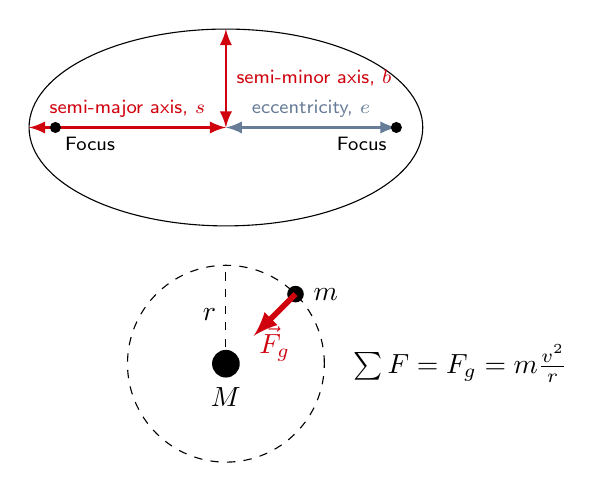
\begin{tikzpicture}
\tikzmath{
\a=2.5;
\b=1.25;
\c=sqrt(\a*\a-\b*\b);
\xe=\a/2;
\ye=\b/2*sqrt(3);
\ae=0.5*\a;
\be=0.7*\b;
\ce=sqrt(\ae*\ae-\be*\be);
\xm=\xe+\ce+\ae/2;
\ym=\ye+\be/2*sqrt(3);
}

\scalebox{1}{
\draw (0,0) ellipse ({\a} and \b);

\draw[latex-latex, line width=1,color=myred] (0,0) -- +(0,\b) node[midway,right]{\scriptsize semi-minor axis, $b$};
\draw[latex-latex, line width=1,color=myred] (0,0) -- +(-\a,0) node[midway,above]{\scriptsize semi-major axis, $s$};
\draw[latex-latex, line width=1,color=myblue!60] (0,0) -- +(\c,0) node[midway,above]{\scriptsize eccentricity, $e$};
\fill (-\c,0) circle(2pt) node[below right]{\scriptsize Focus};
\fill (\c,0) circle(2pt) node[below left]{\scriptsize Focus};


\begin{scope}[shift={(0,-3)}]
\only<2->{
\draw[dashed] (0,0) circle (0.5*\a);

\fill (45:0.5*\a) circle (3pt) node[right=3pt]{$m$};
\fill (0,0) circle (5pt) node[below=5pt]{$M$};
\draw[dashed] (0,0) -- (90:0.5*\a) node[midway,left]{$r$};
\draw [-latex, line width=2,color=myred] (45:0.5*\a) -- +(225:0.3*\a)node[midway,below]{$\vec F_g$};
\node[right] at (0.6*\a,0) {$\sum F=F_g=m\frac{v^2}{r}$};
}
\end{scope}

}

\end{tikzpicture}
\only<2->{
\captionof*{figure}{\textit{For a circular orbit, the semi-major axis is just the radius. The force of gravity is responsible for the radial acceleration.}}
}
\end{center}

}








%%%%%%%%%%%%%%%%%%%%%

\section{The Gravitational Field and Gauss' Law}
\label{sec:gravfieldandgauss}
\title{The Gravitational Field and Gauss' Law}


%%%%%%%%%%%%%%%%%%%%%%%%%
\begin{frame}
\titlepage
\thispagestyle{empty}
\end{frame}

%%%%%%%%%%%%%%%%%%%%%%








%%%%%%%%%%%%%%%%%%%%%%%%
\subsection{Apparent weight}
\label{subsec:apparentweight}
\twocolframesf{Apparent weight}
{
\begin{itemize}
\item Can be defined as \textbf{the net force ($\sum \vec F$) on you minus the force of gravity}.
\item If you stand on a scale, the only 2 forces exerted on you are gravity and the normal force:
\begin{itemize}
\item[$\rightarrow$] The normal force is your apparent weight:
\begin{align*}
\sum \vec F &= \vec F_g+\vec N\\
\vec W &=\sum \vec F - \vec F_g = \vec N
\end{align*}

\item[$\rightarrow$] The scale measures the magnitude of the normal force.
\end{itemize}

\item You feel ``weightless'' when your apparent weight is zero, \textbf{not} when you have no weight.
\end{itemize}
}
{
\begin{center}
\begin{tikzpicture}
\tikzmath{
\L=5;
\w=3;
}

\scalebox{1}{

\draw[line width=1.5] (0,0) rectangle (\w,\L);
\node at (0.25*\w,0.45*\L) {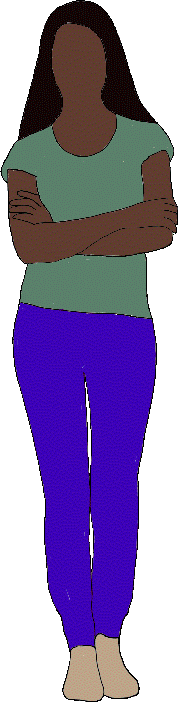
\includegraphics[scale=0.15]{figures/Gravity/woman}} ;
\draw[line width=1.5] (0.1*\w,0.05) rectangle (0.45*\w,0.07*\L);
\node at (0.27*\w,0.035*\L){\scriptsize $W$};
\fill (0.75*\w,0.5*\L) circle (2pt);
\draw[-latex, line width=1.5] (0.75*\w,0.5*\L) -- +(0,1.4) node[midway,right]{$\vec N$};
\draw[-latex, line width=1.5] (0.75*\w,0.5*\L) -- +(0,-1) node[midway,right]{$\vec F_g$};
\draw[-latex, line width=5, color=myred] (1.25*\w,0.4*\L) -- +(0,1.3) node[midway,right]{$\vec a$};
}

\end{tikzpicture}
\captionof*{figure}{\textit{A person on a scale in an elevator accelerating upwards. The scale reads the value of the apparent weight, which is equal to the normal force.}}
\end{center}

}


%%%%%%%%%%%%%%%%%%%%%%%%%%%%%%%%



%%%%%%%%%%%%%%%%%%%%%%%%%%%%%%%%
\twocolframesf{Apparent weight on Earth}
{
\only<1>{
\begin{itemize}
\item At the North Pole, you are not accelerating, so the normal force has the same magnitude as your weight.
\item At the equator, you are accelerating towards the centre of the Earth (uniform circular motion) – the normal force is thus smaller,
\item The effect is small...
\begin{align*}
\vec W &=\sum \vec F - \vec F_g = \vec N\\
\sum F_r&=F_g-N=m\frac{v^2}{R}\\
W&=N=mg=mg-m\frac{v^2}{R}=m\left(g- \frac{v^2}{R} \right)
\end{align*}
\end{itemize}
}
\only<2>{
\begin{itemize}
\item Your apparent weight depends on how fast you rotate about the centre of the Earth:
\begin{align*}
W=m\left(g- \frac{v^2}{R} \right)
\end{align*}
\item If you go just the right speed, your apparent weight will be zero:
\item This is what being ``weightless'' means.
\item If your acceleration is $g$, then you feel weightless. If the only force exerted on you is that from gravity, you feel weightless. 
\end{itemize}
}
}
{
\vspace{-1cm}
\begin{center}
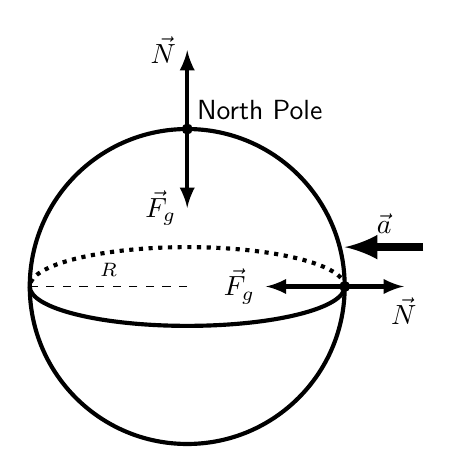
\begin{tikzpicture}
\tikzmath{
\R=2;
}

\scalebox{1}{
\coordinate (P1) at (1.0*\R,0);
\coordinate (P2) at (0,1.0*\R);

\draw[line width=1.5] (0,0) circle (\R);
\draw[dotted, line width=1.5] (\R,0) arc(0:180:{\R} and {\R/4});
\draw[line width=1.5] (\R,0) arc(0:-180:{\R} and {\R/4});
\draw[dashed] (0,0) -- (-\R,0) node[midway,above]{\scriptsize $R$};

\fill (P1) circle (2pt) ;
\draw[-latex,line width=1.5] (P1) -- +(-1,0) node[left]{$\vec F_g$};
\draw[-latex,line width=1.5] (P1) -- +(0.75,0) node[below]{$\vec N$};
\draw[-latex, line width=3] ($(P1)+(1,0.5)$) -- +(-1,0) node[midway,above]{$\vec a$};

\fill (P2) circle (2pt)node[above right]{North Pole};
\draw[-latex,line width=1.5] (P2) -- +(0,-1) node[left]{$\vec F_g$};
\draw[-latex,line width=1.5] (P2) -- +(0,1) node[left]{$\vec N$};


}

\end{tikzpicture}
\captionof*{figure}{\textit{Apparent weight on a rotating Earth. The normal force is smaller at the equator since some of the weight contributes to the centripetal acceleration.}}
\end{center}

}


%%%%%%%%%%%%%%%%%%%%%%%%%%%%%%%%
\twocolframesf{A plumb line}
{

\begin{itemize}
\item We use plumb lines to determine the vertical direction.
\item The mass on the plumb line accelerates with the Earth, so the net force on it is not zero (and the tension is thus not opposite of gravity). The line does not point to the centre of the Earth (except at Pole/Equator).
\item If you cut the line, it’s a little complicated, since the mass does not have an initial speed of zero (as it rotates around the Earth) \url{http://articles.adsabs.harvard.edu/pdf/1897PA......5..186W}
\item The effect is very small for the Earth.
\end{itemize}

}
{

\begin{center}
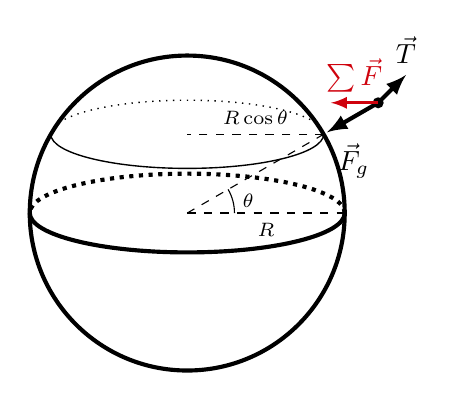
\begin{tikzpicture}
\tikzmath{
\R=2;
\Rc=\R*cos(30);
}

\scalebox{1}{
\coordinate (P) at (30:1.4*\R);


\draw[line width=1.5] (0,0) circle (\R);
\draw[dotted, line width=1.5] (\R,0) arc(0:180:{\R} and {\R/4});
\draw[line width=1.5] (\R,0) arc(0:-180:{\R} and {\R/4});
\draw[dashed] (0,0) -- (\R,0) node[midway,below]{\scriptsize $R$};

\fill (P) circle (2pt) ;
\draw[-latex,line width=1.5] (P) -- +(210:0.75)node[below right]{$\vec F_g$};
\draw[-latex,line width=1.5] (P) -- +(45:0.5)node[above]{$\vec T$};
\draw[-latex,line width=1, color=myred] (P) -- +(180:0.6)node[midway,above]{$\sum \vec F$};

\draw[dotted, line width=0.5] (30:\R) arc(0:180:{\Rc} and {\Rc/4});
\draw[line width=0.5] (30:\R) arc(0:-180:{\Rc} and {\Rc/4});
\draw[dashed] (30:\R) -- +(-\Rc,0) node[midway,above]{\scriptsize $R\cos\theta$};
\draw[dashed] (0,0) -- (30:\R);
\draw (0.3*\R,0) arc (0:30:0.3*\R) node[midway,right]{\scriptsize $\theta$};
}

\end{tikzpicture}
\captionof*{figure}{\textit{Except at the poles and equator, a plumb line does not point towards the centre of the Earth!}}
\end{center}

}


%%%%%%%%%%%%%%%%%%%%%%%%%%%%%%%%
\subsection{Gravitational field}
\label{subsec:gravitationalfield}
\begin{frame}{Gravitational field}
\begin{itemize}
\item Near the centre of the Earth, we use the force of gravity as:
\begin{align*}
\vec F_g=m\vec g
\end{align*}
\item We call, $\vec g$, the \textbf{gravitational field} of the Earth (rather than the acceleration due to gravity).
\item This has to be the same as the force from Newton's Theory of Gravity:
\begin{align*}
F_g=G\frac{Mm}{R^2}
\end{align*}
\item Thus, in terms of the mass (M) and radius (R) of the Earth, the gravitational field at the surface of the Earth is:
\begin{align*}
g=\frac{F_g}{m}=G\frac{M}{R^2}
\end{align*}
\end{itemize}
\end{frame}


%%%%%%%%%%%%%%%%%%%%%%%%%%%%%%%%
\twocolframesf{Gravitational field, $\vec g$}
{
\begin{itemize}
\item The force on $m$ from $M$:
\begin{align*}
\vec F(\vec r)=-G\frac{Mm}{r^2}\hat r
\end{align*}
\item The force from $M$ \textbf{per unit mass} is called the gravitational field of $M$:
\begin{align*}
\vec g(\vec r)=\frac{\vec F(\vec r)}{m}=-G\frac{M}{r^2}\hat r
\end{align*}
\item The gravitational field is associated with $M$, and makes it easy to calculate the force from $M$ on any mass, $m’$:
\begin{align*}
\vec F'(\vec r)=m'\vec g(\vec r)
\end{align*}
\end{itemize}
}
{
\begin{center}
\begin{tikzpicture}
\scalebox{0.8}{
%Simple way to do a 1/r^2 vector field:
\foreach \x in {-3,-2.5,-2,-1.5,-1,-0.5,0,0.5,1,1.5,2,2.5,3}{%don't need this to be an array...
\foreach \y in {-3,-2.5,-2,-1.5,-1,-0.5,0,0.5,1,1.5,2,2.5,3}{
\tikzmath{
\r=\x*\x+\y*\y+0.001;
\dx=-\x/\r;
\dy=-\y/\r;
}
%ATTENTION: NEED LENGTHTEST to trick it to use float, ifthenelse only works with ints!!!
\ifthenelse{\lengthtest{\r pt> 1.5pt}}{\draw[-latex] (\x,\y) --+(\dx,\dy);}{};
}

}
\node at (0,0){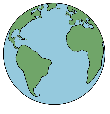
\includegraphics[scale=0.5]{figures/Gravity/earth}};
}

\end{tikzpicture}
\captionof*{figure}{\textit{Gravitational field vectors around the Earth.}}
\end{center}
}


%%%%%%%%%%%%%%%%%%%%%%%%%%%%%%%%
\subsubsection{Field lines}
\label{subsubsec:fieldlines}
\twocolframesf{Visualizing the gravitational field: field lines}
{
\begin{itemize}
\item If you have a mass M in space, one can think of the gravitational field as existing everywhere in space around M.
\item We can visualize this with \textbf{field lines}.
\item The gravitational field vector is in the \textbf{direction tangent to the field line} and has a \textbf{magnitude proportional to the density of field lines}.
\item Near the surface of the Earth, these are parallel lines downwards.
\end{itemize}
}
{
\vspace{-0.75cm}
\begin{center}
\begin{tikzpicture}
\tikzmath{
\L=3;
}
\scalebox{1}{

\begin{scope}
\clip (-0.6*\L,-0.6*\L) rectangle (0.6*\L,0.6*\L);
\foreach \th in {0,10,...,360}{
\draw (0,0) -- (\th:\L);
\draw[-latex] (\th:0.4*\L) -- +(\th:-0.2);
}
\end{scope}
\node at (0,0){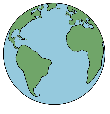
\includegraphics[scale=0.3]{figures/Gravity/earth}};
\draw[-latex,line width=1.5,color=myred] (40:0.75*\L) -- +(40:-0.15*\L);
\draw[-latex,line width=1.5,color=myred] (-40:0.4*\L) -- +(-40:-0.25*\L);

\begin{scope}[shift={(0,-1.25*\L)}]

\foreach \x in {-0.5, -0.4,...,0.6}{
 \draw (\x*\L,0) -- +(0,0.5*\L);
 \draw[-latex] (\x*\L,0.25*\L) -- +(0,-0.2);
}
\fill[color=brown] (-0.5*\L,0) rectangle (0.5*\L,0.1);
\end{scope}

}

\end{tikzpicture}
\captionof*{figure}{\textit{Gravitational field lines around the Earth. Close to the surface, they are effectively parallel, so the field is essentially constant.}}
\end{center}
}


%%%%%%%%%%%%%%%%%%%%%%%%%%%%%%%%
\subsubsection{Superposition principle}
\label{subsubsec:superpositionprinciple}
\twocolframesf{The Superposition Principle}
{
\begin{itemize}
\item If there are two bodies, say $M_1$ and $M_2$, we can calculate the field from each body separately.
\item The total gravitational field at some point in space is then the sum of the individual gravitational fields.
\item If you calculate the net force on a satellite from both the Earth and Moon, you would add the force vectors. Since the g-field is just the force per unit mass, you can add those together as well.
\item The field from the Moon does not depend on the field from the Earth (superposition).
\end{itemize}
}
{
\begin{center}
\begin{tikzpicture}
\tikzmath{
\xe=-2;%Coordinates of first mass/charge (Earth)
\ye=0;
\xm=2;%Coordinates of first mass/charge (Moon)
\ym=0;
\mee=1;% Mass/charge of first mass (Earth)
\mmm=0.6;% Mass/charge of first mass (Earth)
\dl=0.1;%scale factor to advance along the field line
\n=35;%number of points to find in the line (make as small as possible to reach the point you want!)
}

\scalebox{1}{
%Top field lines (xst is the starting x position of the field line)
\foreach \xst in {-1,-0.8,...,1}{
  \tikzmath{
  \yst=1.5; %all field lines start at yst
  \x=\xst;
  \y=\yst;
  %
  %generate points on the line (keeps finding the next point)
  int \i;
  %note that this also creates \mypairx and \mypairy!
  coordinate \mypair;
  for \i in {1,...,\n}{
    %First mass (earth)
    \re=(\x-\xe)*(\x-\xe)+(\y-\ye)*(\y-\ye)+0.0001;
    \Fex=-\mee*(\x-\xe)/\re;
    \Fey=-\mee*(\y-\ye)/\re;
    %Second mass (moon)
    \rm=(\x-\xm)*(\x-\xm)+(\y-\ym)*(\y-\ym)+0.0001;
    \Fmx=-\mmm*(\x-\xm)/\rm;
    \Fmy=-\mmm*(\y-\ym)/\rm;
    %Total force:
    \Fx=\Fex+\Fmx;
    \Fy=\Fey+\Fmy;
    \Fn=sqrt(\Fx*\Fx+\Fy*\Fy)+0.0001;
    \dx=\Fx/\Fn*\dl;
    \dy=\Fy/\Fn*\dl;
    \x=\x+\dx;
    \y=\y+\dy;
    \mypair{\i}=(\x,\y);
    };
  }
  %Draw that field line
  \foreach \i in {2,...,\n}{
    \tikzmath{
    int \im;
    \im=\i-1;
    }
    \draw (\mypair{\im}) -- (\mypair{\i});
    \ifthenelse{\im =5}{\draw[-latex] (\mypair{\im}) -- (\mypair{\i})}{};%draw arrow on the fifth point
  }

}%end of loop over x

%Bottom field lines
\foreach \xst in {-1,-0.8,...,1}{
  \tikzmath{
  \yst=-1.5;
  \x=\xst;
  \y=\yst;
  %
  %generate points on the line
  int \i;
  %note that this also creates \mypairx and \mypairy!
  coordinate \mypair;
  for \i in {1,...,\n}{
    %First mass (earth)
    \re=(\x-\xe)*(\x-\xe)+(\y-\ye)*(\y-\ye)+0.0001;
    \Fex=-\mee*(\x-\xe)/\re;
    \Fey=-\mee*(\y-\ye)/\re;
    %Second mass (moon)
    \rm=(\x-\xm)*(\x-\xm)+(\y-\ym)*(\y-\ym)+0.0001;
    \Fmx=-\mmm*(\x-\xm)/\rm;
    \Fmy=-\mmm*(\y-\ym)/\rm;
    %Total force:
    \Fx=\Fex+\Fmx;
    \Fy=\Fey+\Fmy;
    \Fn=sqrt(\Fx*\Fx+\Fy*\Fy)+0.0001;
    \dx=\Fx/\Fn*\dl;
    \dy=\Fy/\Fn*\dl;
    \x=\x+\dx;
    \y=\y+\dy;
    \mypair{\i}=(\x,\y);
    };
  }
  %Draw that field line
  \foreach \i in {2,...,\n}{
    \tikzmath{
    int \im;
    \im=\i-1;
    }
    \draw (\mypair{\im}) -- (\mypair{\i});
    \ifthenelse{\im =5}{\draw[-latex] (\mypair{\im}) -- (\mypair{\i})}{};
  }

}%end of loop over x

%Draw the Earth, Moon and example point
\node at (\xe,\ye) {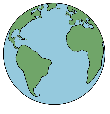
\includegraphics[scale=0.3]{figures/Gravity/earth}};
\node at (\xm,\ym) {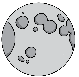
\includegraphics[scale=0.3]{figures/Gravity/moon}};

%Calculate field vector directions
\tikzmath{
    \xp=1.5;
    \yp=2;
    \fscale=2.5;
    \re=(\xp-\xe)*(\xp-\xe)+(\yp-\ye)*(\yp-\ye)+0.0001;
    \Fex=-\mee*(\xp-\xe)/\re;
    \Fey=-\mee*(\yp-\ye)/\re;
    %Second mass (moon)
    \rm=(\xp-\xm)*(\xp-\xm)+(\yp-\ym)*(\yp-\ym)+0.0001;
    \Fmx=-\mmm*(\xp-\xm)/\rm;
    \Fmy=-\mmm*(\yp-\ym)/\rm;
    %Total force:
    \Fx=\Fex+\Fmx;
    \Fy=\Fey+\Fmy;
    \Fn=sqrt(\Fx*\Fx+\Fy*\Fy)+0.0001;
    \dx=\Fx/\Fn;
    \dy=\Fy/\Fn;
}
\coordinate (P) at (\xp,\yp);
\fill (P) circle(2pt);
\draw[-latex,line width=1] (P) -- +(\fscale*\Fex,\fscale*\Fey) node[above left]{$\vec g_{Earth}$};
\draw[-latex,line width=1] (P) -- +(\fscale*\Fmx,\fscale*\Fmy) node[right]{$\vec g_{Moon}$};
\draw[-latex,line width=1,color=myred] (P) -- +(\fscale*\Fx,\fscale*\Fy) node[below right]{$\vec g_{tot}$};
}

\end{tikzpicture}
\captionof*{figure}{\textit{Gravitational field lines for an Earth-Moon system.}}
\end{center}
}




%%%%%%%%%%%%%%%%%%%%%%%%%%%%%%%%


%%%%%%%%%%%%%%%%%%%%%%%%%%%%%%%%
\subsection{Gauss' law}
\label{subsec:gausslaw}
\begin{frame}{Gauss' Law}
\begin{itemize}
\item Gauss' Law allows us to calculate the magnitude of the gravitational field in situations with high symmetry.
\item \textbf{Newton's Universal Law of Gravity is only valid for point masses} (most masses, like the Earth, are not a point mass) – How would you calculate the gravitational field/force at a location half-way inside the Earth?
\item It is a consequence of Gauss' Law that we can model the Earth as a point mass, with all the mass at the centre of the Earth, if we want to calculate the force of gravity/gravitational field \textbf{outside} of the Earth.	
\end{itemize}

\end{frame}


%%%%%%%%%%%%%%%%%%%%%%%%%%%%%%%%
\subsubsection{Theory}
\label{subsubsec:gausstheory}
\begin{frame}{Gauss' Law - The basic idea}
\begin{center}
\begin{tikzpicture}
\tikzmath{
\L=3;
\R=0.75;
}
\scalebox{1}{

\begin{scope}
\clip (-0.6*\L,-0.6*\L) rectangle (0.6*\L,0.6*\L);
\foreach \th in {0,20,...,360}{
\draw (0,0) -- (\th:\L);
\draw[-latex] (\th:0.4*\L) -- +(\th:-0.2);
}
\end{scope}
\node at (0,0){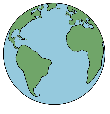
\includegraphics[scale=0.3]{figures/Gravity/earth}};

\only<2>{
\shade[ball color=myred, opacity=0.5] (0,0) circle (\R);
\draw[line width=1.5, color=myred, opacity=0.5] (\R,0) arc(0:-180:{\R} and {\R/4});
\node[color=myred] at (50:1.5*\R){$S$};
}

}

\end{tikzpicture}
\captionof*{figure}{\textit{Gravitational field lines around the Earth.\only<2>{ Enclosing the Earth with a gaussian spherical surface, $S$.}}}
\end{center}

\begin{itemize}
\item If you \textbf{enclose} a mass with a surface, $S$, then the number of field lines that cross that surface depends on the mass that you’ve enclosed.
\item<2> Makes sense, if you have a heavier mass, you have a denser field lines, so more of them will enter $S$.
\end{itemize}

\end{frame}


%%%%%%%%%%%%%%%%%%%%%%%%%%%%%%%%
\subsubsection{Formula}
\label{subsubsec:gaussformula}
\begin{frame}{Gauss' Law}
\begin{align*}
\oint \vec g(\vec r) \cdot d\vec A=4\pi G M^{enc}
\end{align*}

\begin{itemize}
\item Two sides to the equation:
\begin{enumerate}
\item Left side: \textbf{flux of the field through the surface}. It is a measure of the number of field lines through the surface.
\item Right-side: amount of \textbf{mass enclosed by the surface} that \textit{we chose}.
\end{enumerate}
\item The flux is a ``surface integral'' over a closed surface. It is the sum of the dot products of the field, $\vec g(\vec r)$ , with a vector, $d\vec A$, that is always normal to the surface.
\item To use Gauss' Law:
\begin{enumerate}
\item Choose a closed surface and figure out how much mass is inside.
\item Figure out how much flux is coming out the surface.
\item Set them equal and determine, say, the gravitational field.
\end{enumerate}
\item Gauss' Law is most useful in situations with a high degree of symmetry (e.g. spherical symmetry).
\end{itemize}
\end{frame}


%%%%%%%%%%%%%%%%%%%%%%%%%%%%%%%%
\subsubsection{Field outside a uniform sphere}
\label{subsubsec:fieldoutsidesphere}
\twocolframesf{Field outside of a uniform sphere of radius, $R$, and mass, $M$}
{
Want the field, $\vec g(\vec r)$, at some distance $r$ from the centre:
\begin{itemize}
\item[1]<2-> Choose a spherical surface ($S$) of radius $r$.
\only<3,4>{
\item[2] Evaluate the flux integral (use symmetry arguments):
\begin{align*}
\oint \vec g(\vec r) \cdot d\vec A=-\oint g(r) dA=-g(r) \oint dA
\end{align*}
\item[$\rightarrow$]<4> Adding together all of the $dA$:
\begin{align*}
\oint dA&=4\pi r^2\\
\therefore \oint \vec g(\vec r) \cdot d\vec A&=-4\pi r^2 g(r)
\end{align*}
}
\only<5>{
\item[2] Evaluate the flux integral: $-4\pi r^2 g(r)$
\item[3] Determine the mass enclosed. In this case, all of $M$ is enclosed:
\begin{align*}
M^{enc}=M
\end{align*}
}
\only<6>{
\item[2] Evaluate the flux integral: $-4\pi r^2 g(r)$
\item[3] Determine the mass enclosed: $M^{enc}=M$
\item[4] Put it all together:
\begin{align*}
\oint \vec g(\vec r) \cdot d\vec A&=4\pi G M^{enc}\\
-4\pi r^2 g(r) &= 4\pi G M \\
\therefore g(r)&=-G\frac{M}{r^2}
\end{align*}
}
\end{itemize}

}
{
\begin{center}
\begin{tikzpicture}
\tikzmath{
\Rm=0.3;
\Rs=1.5;
}
\scalebox{1}{

\shade[ball color=myblue!60] (0,0,0) circle (\Rm);
\only<1>{\node at (-45:2.5*\Rm) {\scriptsize $M,R$};}
\fill (-\Rs,0) circle(2pt);
\draw[dashed,line width=1] (0,0) -- (-\Rs,0) node[midway,above]{$r$};

\only<2->{
\draw[-latex, line width=1] (45:0.775*\Rs) -- +(45:-0.75) node[right=5pt]{$\vec g$};
\shade[ball color=myred, opacity=0.25] (0,0,0) circle (\Rs);
\draw[line width=1.5, color=myred, opacity=0.5] (\Rs,0) arc(0:-180:{\Rs} and {\Rs/4});
\node[color=myred] at (135:1.5*\Rs){$S$};

\fill[color=myred,opacity=0.5, draw=black] (35:0.7*\Rs) -- (37.5:0.85*\Rs) -- (52.5:0.85*\Rs) -- (55:0.7*\Rs) --cycle;
\draw[-latex,color=myred, line width=1] (45:0.775*\Rs) -- +(45:0.75) node[right]{$d\vec A$};
}
}
\end{tikzpicture}
\captionof*{figure}{\textit{Gauss' Law to find field outside of a spherical mass of radius, $R$, and mass, $M$.}}
\end{center}
}


%%%%%%%%%%%%%%%%%%%%%%%%%%%%%%%%
\subsubsection{Field inside a uniform sphere}
\label{subsubsec:fieldinsidesphere}
\twocolframesf{Field \textit{inside} of a uniform sphere of radius, $R$, and mass, $M$}
{
Want the field, $\vec g(\vec r)$, at some distance $r<R$ from the centre:
\begin{itemize}
\item[1]<2-> Choose a spherical surface ($S$) of radius $r$.
\only<3>{
\item[2] Evaluate the flux integral (same as before):
\begin{align*}
\oint \vec g(\vec r) \cdot d\vec A&=-\oint g(r) dA=-g(r) \oint dA\\
&=-4\pi r^2 g(r)
\end{align*}
}
\only<4>{
\item[2] Evaluate the flux integral: $-4\pi r^2 g(r)$
\item[3] Determine the mass enclosed. Use the density, $\rho=\frac{M}{V}$:
\begin{align*}
\rho&=\frac{M}{\frac{4}{3}\pi R^3}\\
M^{enc}&=\rho \frac{4}{3}\pi r^3=\frac{M}{\frac{4}{3}\pi R^3}\frac{4}{3}\pi r^3\\
&=M\frac{r^3}{R^3}
\end{align*}
}
\only<5>{
\item[2] Evaluate the flux integral: $-4\pi r^2 g(r)$
\item[3] Determine the mass enclosed: $M^{enc}=M\frac{r^3}{R^3}$
\item[4] Put it all together:
\begin{align*}
\oint \vec g(\vec r) \cdot d\vec A&=4\pi G M^{enc}\\
-4\pi r^2 g(r) &= 4\pi G M\frac{r^3}{R^3} \\
\therefore g(r)&=-G\frac{M}{R^3}r
\end{align*}
}
\end{itemize}

}
{
\begin{center}
\begin{tikzpicture}
\tikzmath{
\Rm=2;
\Rs=1.25;
}
\scalebox{1}{
\draw[dashed,line width=1] (0,0) -- (-\Rs,0) node[midway,above]{$r$};
\fill (-\Rs,0) circle(2pt);
\only<1>{
\shade[ball color=myblue!60,opacity=0.5] (0,0,0) circle (\Rm);
}
\node at (-45:1.15*\Rm) {\scriptsize $M,R$};



\only<2->{


\draw[-latex, line width=1] (45:0.775*\Rs) -- +(45:-0.75) node[right=5pt]{$\vec g$};
\shade[ball color=myred, opacity=0.25] (0,0,0) circle (\Rs);
\draw[line width=1.5, color=myred, opacity=0.5] (\Rs,0) arc(0:-180:{\Rs} and {\Rs/4});
\node[color=myred] at (135:1.25*\Rs){$S$};

\fill[color=myred,opacity=0.6, draw=black] (35:0.7*\Rs) -- (37.5:0.85*\Rs) -- (52.5:0.85*\Rs) -- (55:0.7*\Rs) --cycle;

\draw[-latex,color=myred, line width=1] (45:0.775*\Rs) -- +(45:0.75) node[right]{$d\vec A$};
\shade[ball color=myblue!60,opacity=0.5] (0,0,0) circle (\Rm);
}

}

\end{tikzpicture}
\captionof*{figure}{\textit{Gauss' Law to find field inside of a spherical mass of radius, $R$, and mass, $M$.}}
\end{center}
\only<5>{
Inside the sphere, the field increases linearly with radius. Outside it decreases with $r^2$.
}
}


%%%%%%%%%%%%%%%%%%%%%%%%%%%%%%%%










%%%%%%%%%%%%%%%%%%%%%

\section{Gravitational Potential and General Relativity}
\label{sec:gravpotentialandgr}
\title{Gravitational Potential and General Relativity}
\institute{Gravity}
\author{\insertsubsection}


%%%%%%%%%%%%%%%%%%%%%%%%%
\begin{frame}
\titlepage
\thispagestyle{empty}
\end{frame}

%%%%%%%%%%%%%%%%%%%%%%











%%%%%%%%%%%%%%%%%%%%%%%%%%%%%%%%
\subsection{Gravitational potential energy}
\label{subsec:gravitationalpotentialenergy}
\twocolframe{Gravitational potential energy}
{
\begin{itemize}
\item The force exerted on mass $m$ from mass $M$:
\begin{align*}
\vec F = - G \frac{Mm}{r^2}\hat r= - G \frac{Mm}{r^3}\vec r
\end{align*}
\item To determine the change in potential energy, we need to calculate the work done along a particular path:
\begin{align*}
W&=\int_A^B\vec F \cdot d\vec l\\
\Delta U &= U(\vec r_B)-U(\vec r_A)
\end{align*}
\end{itemize}

}
{
\begin{center}
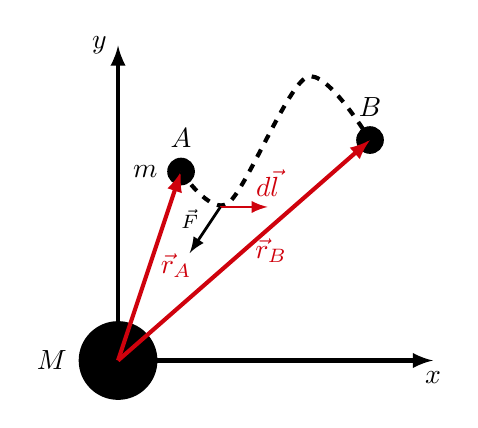
\begin{tikzpicture}
\tikzmath{
\L=4;
}
\scalebox{1}{

\coordinate (M) at (0,0);
\coordinate (mA) at (0.2*\L, 0.6*\L);
\coordinate (mB) at (0.8*\L, 0.7*\L);
\coordinate (P1) at (0.35*\L, 0.5*\L);
\coordinate (P1a) at ($(P1)-(0.1,0.05)$);
\coordinate (P2) at (0.6*\L, 0.9*\L);

\draw[-latex,line width=1.5] (0,0) -- (\L,0) node[below]{$x$};
\draw[-latex,line width=1.5] (0,0) -- (0,\L) node[left]{$y$};

\fill (M) circle (0.5) node[left=15pt]{$M$};
\fill (mA) circle (5pt) node[left=5pt]{$m$} node[above=5pt]{$A$};
\fill (mB) circle (5pt) node[above=5pt]{$B$};

\draw[color=myred,-latex,line width=1.5] (M) -- (mA) node[midway,right] {$\vec r_A$};
\draw[color=myred,-latex,line width=1.5] (M) -- (mB) node[midway,right] {$\vec r_B$};

\draw[line width=1.5, dashed] plot [smooth] coordinates {(mA) (P1) (P2) (mB)};

\draw[-latex, color=myred, line width = 1] (P1a) -- +(0.6,0) node[above]{$d \vec l$};
\draw[-latex, line width = 1] (P1a) -- ($(P1a)!0.3!(0,0)$) node[above=5pt]{\scriptsize $\vec F$};
}
\end{tikzpicture}
\captionof*{figure}{\textit{The work done by gravity on mass $m$ in going from $A$ to $B$, depends only on the end points.}}
\end{center}

}


%%%%%%%%%%%%%%%%%%%%%%%%%%%%%%%%
\subsubsection{Determining the potential}
\label{subsubsec:determiningthepotential}
\twocolframesf{Determining the gravitational potential energy function, $U(\vec r)$}
{
\begin{itemize}
\item Choose straight line as a path, to make it 1D (and our lives easier):
\begin{align*}
\only<1->{
W&=\int _{r_A}^{r_B} \vec F\cdot d\vec r=\int _{r_A}^{r_B} F(r) dr=\int _{r_A}^{r_B} -G\frac{Mm}{r^2} dr\\
}
\only<2->{
&=\left[ G\frac{Mm}{r}  \right] _{r_A}^{r_B} = G\frac{Mm}{r_B}-G\frac{Mm}{r_A}=\textcolor{myred}{-}\Delta U 
}
\end{align*}
\item<3-> By inspection:
\begin{align*}
\Delta U &= G\frac{Mm}{r_A}-G\frac{Mm}{r_B}=U(r_B) - U(r_A)\\
\therefore U&= \textcolor{myred}{-}G\frac{Mm}{r}+C
\end{align*}
\end{itemize}

}
{
\begin{center}
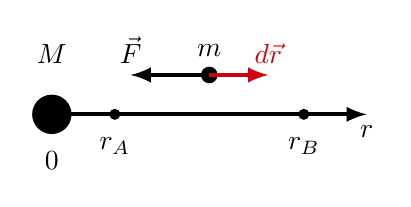
\begin{tikzpicture}
\tikzmath{
\L=4;
}
\scalebox{1}{

\coordinate (M) at (0,0);
\coordinate (mA) at (0.2*\L, 0);
\coordinate (mB) at (0.8*\L, 0);
\coordinate (mid) at ($(mA)!0.5!(mB)+(0,0.5)$);

\draw[-latex,line width=1.5] (0,0) -- (\L,0) node[below]{$r$};

\fill (M) circle (0.25) node[above=15pt]{$M$} node[below=10pt]{$0$};
\fill (mA) circle (2pt) node[below=5pt]{$r_A$};
\fill (mB) circle (2pt) node[below=5pt]{$r_B$};

\fill (mid) circle (3pt) node[above=3pt]{$m$};
\draw[-latex, line width=1.5] (mid) -- +(-1,0) node[above]{$\vec F$};
\draw[-latex, line width=1.5, color=myred] (mid) -- +(0.75,0) node[above]{$d\vec r$};
}
\end{tikzpicture}
\captionof*{figure}{\textit{Calculating the work done on $m$ by gravity along a straight, radial, path, from $r_A$ to $r_B$}}
\end{center}
}


%%%%%%%%%%%%%%%%%%%%%%%%%%%%%%%%
\begin{frame}{Gravitational potential energy}
\begin{itemize}
\item If $m$ is a distance $r$ away from $M$, it will have gravitational potential energy:
\begin{align*}
U&= -G\frac{Mm}{r}+C
\end{align*}
\item A convenient choice of constant is $C = 0$ $\rightarrow$ \textbf{Assume this choice from now on}:
\begin{itemize}
\item[$\rightarrow$] The gravitational potential energy of $m$ becomes 0 when $m$ is infinitely far from $M$ ($r\to\infty$).
\end{itemize}

\end{itemize}

\end{frame}


%%%%%%%%%%%%%%%%%%%%%%%%%%%%%%%%


%%%%%%%%%%%%%%%%%%%%%%%%%%%%%%%%
\subsubsection{Mechanical energy}
\label{subsubsec:mechanicalenergygrav}
\begin{frame}{Mechanical energy}
\begin{itemize}
\item We can define the mechanical energy of $m$, when it is a distance $r$ away from $M$:
\begin{align*}
E=K+U=\frac{1}{2}mv^2-G\frac{Mm}{r}
\end{align*}
\item If gravity is the only force on $m$, then the mechanical energy of $m$ is conserved (constant).
\item This is useful in analyzing possible orbits of $m$ around $M$.
\item As $r\to\infty$, the potential energy goes to zero, and all of the energy must be kinetic.
\end{itemize}
\end{frame}


%%%%%%%%%%%%%%%%%%%%%%%%%%%%%%%%
\subsection{Possible orbits}
\label{subsec:possibleorbits}
\twocolframesf{Possible orbits}
{
\begin{enumerate}
\item If $E<0$, $m$ can never make it to infinity, as kinetic energy would be negative $\rightarrow$ $m$ is ``gravitationally bound'' (as in to bind).
\begin{itemize}
\item If $m$ has the right velocity, it will be in a circular orbit.
\item Otherwise, $m$ will be in an elliptical orbit.
\end{itemize}
\item If $E=0$, $m$ will just barely make it to infinity with zero kinetic energy.
\begin{itemize}
\item This will result in a parabolic orbit.
\item $m$ can ``escape'' the gravitational pull of $M$ (just barely).
\end{itemize}
\item If $E>0$, $m$ will have a non-zero speed when it reaches infinity.
\begin{itemize}
\item The orbit is a hyperbola.
\item $m$ can escape the gravitational pull of $M$.
\end{itemize}

\end{enumerate}
}
{
\begin{center}
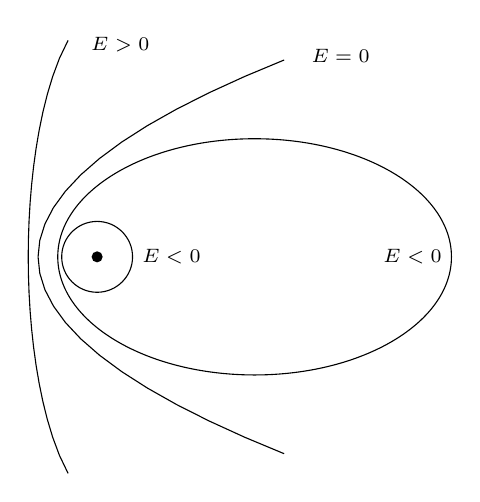
\begin{tikzpicture}
\tikzmath{
\a=2.5;
\b=1.5;
\c=sqrt(\a*\a-\b*\b);
\rc=0.3*\b;
}

\scalebox{1}{
\fill (-\c,0) circle(2pt) ;

\draw (0,0) ellipse ({\a} and \b);
\draw (-\c,0) circle (\rc);

\begin{scope}[rotate=-90,shift={(0,-1.1*\a)}]
\draw plot[domain=-2.5:2.5] (\x,0.5*\x*\x);%parabola
\end{scope}

\begin{scope}[rotate=-90,shift={(0,-0.75*\a)}]
\draw plot[domain=-2.75:2.75] (\x,{-sqrt(1-0.1*\x*\x)});%yperbola
\end{scope}

\node[right] at ($(-\c,0)+(\rc,0)$) {\scriptsize $E<0$};
\node[left] at (\a,0) {\scriptsize $E<0$};
\node[right] at (0.3*\c,1.7*\b) {\scriptsize $E=0$};
\node[right] at (-1.1*\c,1.8*\b) {\scriptsize $E>0$};
}

\end{tikzpicture}
\captionof*{figure}{\textit{Possible orbits depending on energy.}}
\end{center}
}


%%%%%%%%%%%%%%%%%%%%%%%%%%%%%%%%


%%%%%%%%%%%%%%%%%%%%%%%%%%%%%%%%
\subsection{General relativity}
\label{subsec:generalrelativity}
\twocolframesf{Why GR?}
{
\begin{itemize}
\item Newton's Theory does not explain the orbit of Mercury.
\item Newton's Theory is \textbf{fundamentally incompatible} with Special Relativity which requires that no signal can ever travel faster than the speed of light (causality would be violated if something can travel faster than the speed of light).
\end{itemize}
}
{
\capfig{0.8}{figures/Gravity/precession}{Illustration of the precession of Mercury. \tiny\url{https://en.wikipedia.org/wiki/Apsidal_precession}}
}

%%%%%%%%%%%%%%%%%%%%%%%%%%%%%%%%
\twocolframesf{What is GR?}
{
\begin{itemize}
\item Based on the equivalence principle:
\begin{itemize}
\item There’s nothing in physics that requires that the $m$ in $F=ma$ is the same $m$ as in $G\frac{Mm}{r^2}$.
\end{itemize}
\item Really complicated math... ``Differential geometry'':
\begin{align*}
\text{(Curvature)}\quad G_{\mu\nu}=\frac{8\pi G}{c^4}T_{\mu\nu}\quad \text{(Energy)}
\end{align*}
\end{itemize}
Objects are not deflected by the force of gravity. Instead, matter/energy bends space-time so that objects just follow ``straight lines'' in that space. Objects just move inertially (like Newton's first law) through bent space. That is the connection between inertial and gravitational mass.
}
{
\vspace{-1.2cm}
\capfig{0.8}{figures/Gravity/earthfield}{Space time around Earth.}
\vspace{-0.8cm}
\capfig{0.8}{figures/Gravity/membrane}{A simulation of curved space. \tiny\url{http://www.thestargarden.co.uk/General-relativity.html}}
}


%%%%%%%%%%%%%%%%%%%%%%%%%%%%%%%%
\twocolframesf{Some consequences of GR}
{
\begin{itemize}
\item Since light goes in a straight line, and space is curved near a massive object, light will appear to bend around massive objects.
\item Time goes by slower when the gravitational field is stronger (GPS needs to take this into account as time goes by slower near the surface of the Earth than in orbit).
\item The Universe itself is expanding. It’s not expanding into something, space itself is expanding (the distance between stationary objects grows with time).
\item Gravitational waves exist (disturbances in Space Time that propagate like ripples on a pond).
\end{itemize}
}
{
\vspace{-1.2cm}
\capfig{0.8}{figures/Gravity/eddington}{Light bending around the Sun, first successful test of GR. }
\vspace{-0.5cm}
\capfig{0.8}{figures/Gravity/rings}{Einstein rings.}
}


%%%%%%%%%%%%%%%%%%%%%%%%%%%%%%%%
\twocolframesf{Gravitational Waves}
{
\begin{itemize}
\item LIGO experiment recently (2016) detected gravitational waves for the first time $\rightarrow$ 2017 Nobel Prize.
\item It measures distortions in space as a gravitational wave passes by (less than one ten thousandth of the diameter of a proton on a distance of \SI{4}{km}!).
\item The wave was created from an event that released a lot of gravitational potential energy (two black holes falling on each other).
\end{itemize}
}
{
\vspace{-1.5cm}
\begin{center}
\begin{tikzpicture}
\node at (-2cm,0) {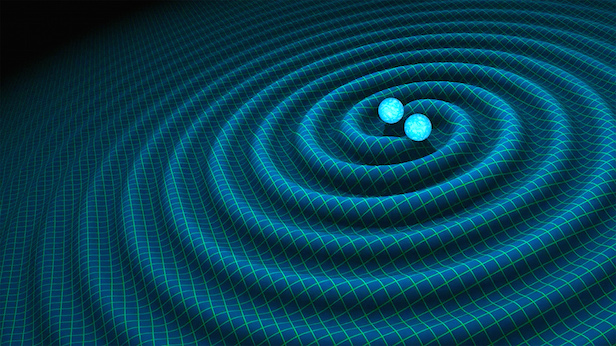
\includegraphics[width=0.8\textwidth]{figures/Gravity/waves}};
\node at (-2cm,-2cm) {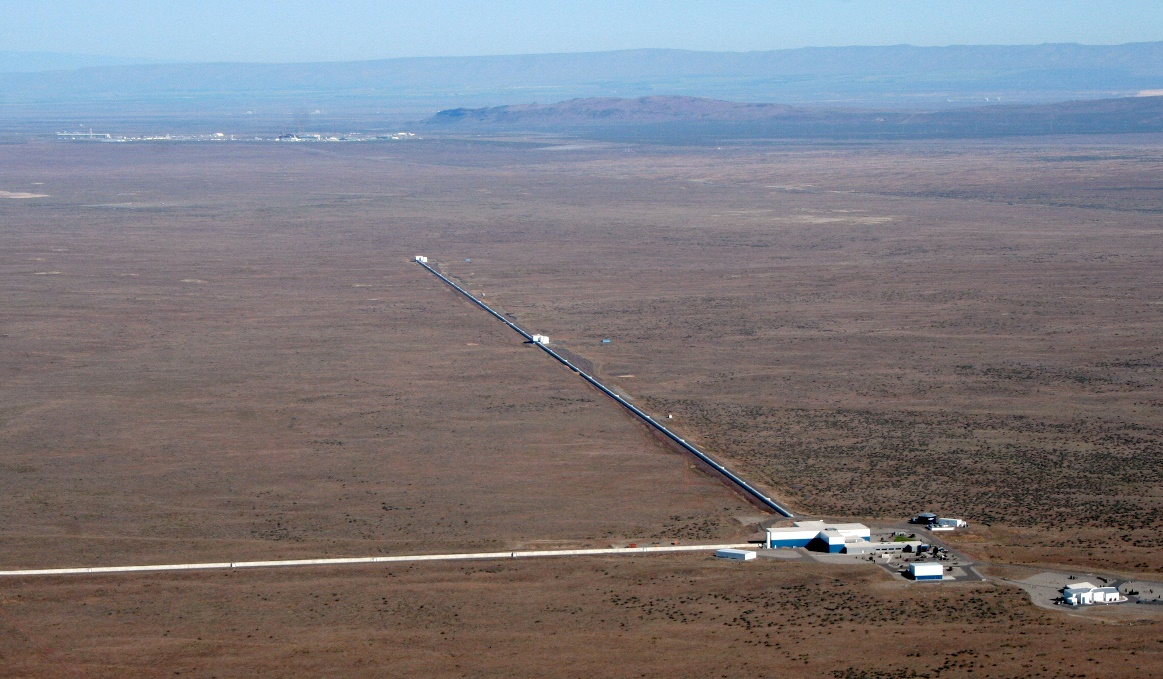
\includegraphics[width=0.8\textwidth]{figures/Gravity/ligo}};
\node at (0.7,-1cm) {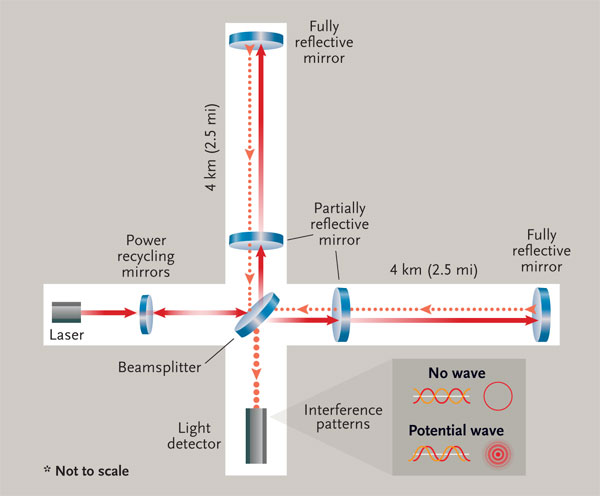
\includegraphics[width=0.45\textwidth]{figures/Gravity/interferometer}};
\end{tikzpicture}
\captionof*{figure}{\textit\tiny{Daw, E. (2016, February 11). Gravitational waves discovered: How did the experiment at LIGO actually work? The Conversation. https://theconversation.com/gravitational-waves-discovered-how-did-the-experiment-at-ligo-actually-work-54510,
\\
Gravitational Wave Detection Heralds New Era. (n.d.). Sky \& Telescope. https://skyandtelescope.org/astronomy-news/gravitational-wave-detection-heralds-new-era-of-science-0211201644}}
\end{center}
}


%%%%%%%%%%%%%%%%%%%%%%%%%%%%%%%%
\begin{frame}{Issues with GR}
\begin{itemize}
\item Mathematically, it is very different from the theories for the other 3 forces of nature – it’s not clear how to combine it into a unified theory of physics (in particular, the ``quantum'' aspect).
\item It has some unusual consequences:
\begin{itemize}
\item Most of the energy (70\%) in the Universe is a ``negative energy'' (``Dark energy'') that is responsible for the Universe expanding $\rightarrow$ we know this from measuring the curvature of space and rate of expansion.
\item Most of the matter in the Universe is in a non-luminous form that we have never detected (``Dark Matter'') $\rightarrow$ we are trying to detect it; we think it's just a different type of particle.
\end{itemize}
\end{itemize}
\end{frame}

%%%%%%%%%%%%%%%%%%%%%%%%%%%%%%%%



%%%%%%%%%%%%%%%%%%%%%%%%%%%%%%%%



%%%%%%%%%%%%%%%%%%%%%%%%%%%%%%%%



%%%%%%%%%%%%%%%%%%%%%%%%%%%%%%%%



%%%%%%%%%%%%%%%%%%%%%%%%%%%%%%%%



%%%%%%%%%%%%%%%%%%%%%%%%%%%%%%%%



%%%%%%%%%%%%%%%%%%%%%%%%%%%%%%%%



%%%%%%%%%%%%%%%%%%%%%%%%%%%%%%%%



%%%%%%%%%%%%%%%%%%%%%%%%%%%%%%%%






\end{document}
